% !TeX root = ../main.tex

\section{Результаты}
\label{sec:results}

\subsection*{Искажение оценок активации и контраста}

При последовательности событий с короткими интервалами и большой разницей амплитуд ОЛМ искажает как отдельные коэффициенты, так и их разность. На рисунке~\ref{fig:f4} показан пример с рассчитанными оценками коэффициентов и контраста, построенный на отдельной серии с высокой плотностью событий. При заданных $a_A=0{,}30$ и $a_B=0{,}05$ ОЛМ занизила оценку большей амплитуды на 27\%, оценку контраста на 36\%. Поправка FV уменьшила снижение амплитуды до 3\%, занижение контраста до 12\%. Поправка FW дала практически тот же контраст, а занижение оценки амплитуды составило 7\%.

При равных заданных амплитудах и нулевом контрасте различие последовательностей предшествующих событий также привело к ненулевой оценке (рис.~\ref{fig:f4}, \textit{b}): стимулы условия A предъявлялись сериями с короткими интервалами, а стимулы B шли с более длинными, поэтому локальное насыщение сильнее подавляло отклик на стимулы A. Поправки FV и FW уменьшили модуль этой оценки примерно на четверть. 

\begin{figure}[!ht]
	\centering
	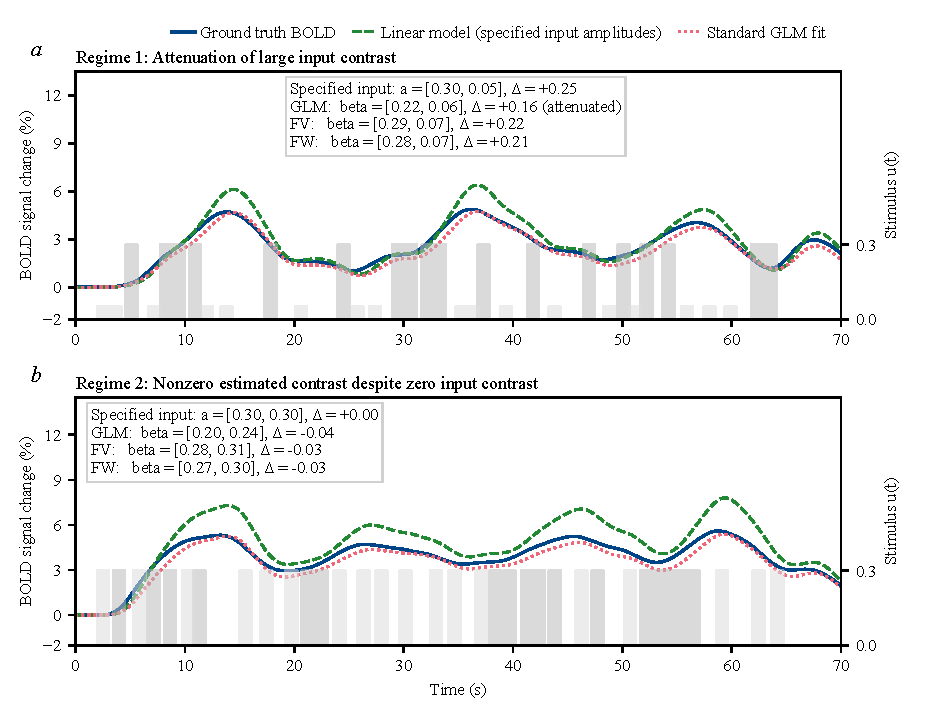
\includegraphics[width=16cm]{fig_4}
	\caption{Два режима нелинейного искажения BOLD-сигнала в последовательностях стимулов: \textit{a} --- занижение контраста при $a_A=0{,}30$, $a_B=0{,}05$ и пуассоновском предъявлении стимулов со средним SOA 1,7~с; \textit{b} --- ненулевая оценка контраста при равных амплитудах $a_A=a_B=0{,}30$ и нулевом заданном контрасте, когда условие A предъявляется с короткими интервалами, а B с более длинными. Сплошная синяя линия --- BOLD-отклик P-DCM, серые столбики на правой оси --- моменты предъявления стимулов условий A и B, зеленый штрих --- линейная модель с канонической HRF при входных амплитудах, красный пунктир --- стандартная оценка ОЛМ; в надписях на панелях --- оценки коэффициентов и контраста для ОЛМ и поправок FV и FW. Запись 70~с, длительность стимула 1~с.}
	\label{fig:f4}
\end{figure}

\subsection*{Форма HRF и ошибка конечных амплитуд}

Собственное линейное приближение проверялось в пределе слабого сигнала: при пиковом приросте потока $0{,}01$ относительная норма $L^2$ разности полного и собственного линейного ответов составляет $0{,}2\%$ и $0{,}3\%$ для P-DCM и BW соответственно. Линейный отклик номинальной P-DCM близок к канонической HRF по положению пика и глубине постстимульного снижения (рис.~\ref{fig:f1}). У BW максимум заметно позже и снижение глубже. 

Однако точность линейного приближения и близость форм не гарантируют точность оценок при конечных амплитудах.
При $L_1$ ошибка контраста сохраняется и растет с амплитудой (рис.~\ref{fig:f5}, табл.~\ref{tab:amp}). В амплитудной бесшумной серии при $a_A=0{,}025$ медианная относительная ошибка у обоих генераторов составляет единицы процентов, а при $a_A=0{,}2$ в последовательностях со средним SOA 2~с достигает четверти контраста. С ростом интервала ошибка уменьшается, но все еще заметна и при SOA 8~с. 

\begin{figure}[!ht]
	\centering
	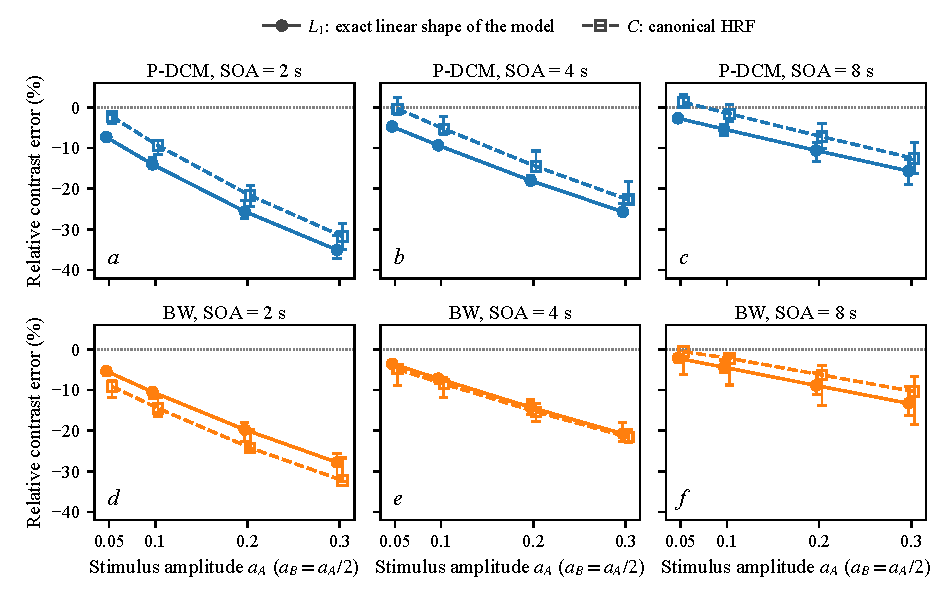
\includegraphics[width=16cm]{fig_5}
	\caption{Относительная ошибка контраста $100(\hat\Delta-\Delta)/\Delta$ при использовании собственного линейного ядра $L_1$ для P-DCM и BW в зависимости от $a_A$ при $a_B=a_A/2$. Рисунки \textit{a}, \textit{b} и \textit{c} соответствуют средним SOA 2, 4 и 8~с; маркеры --- медианы трех последовательностей стимулов, полосы --- описательный разброс min--max между ними.}
	\label{fig:f5}
\end{figure}

\begin{table}[!t]
\captionsetup{justification=raggedright}
\caption{Относительная ошибка контраста: медиана и разброс min--max по последовательностям стимулов; <<все>> --- по девяти последовательностям, отдельные SOA --- по трем последовательностям данного среднего; в амплитудной серии $a_B=0{,}5a_A$, в механистической --- $a_B=0{,}025$}
\label{tab:amp}
\centering
\small
\setlength{\tabcolsep}{4pt}
\begin{tabular}{clccccccc}
\hline
\multirow{2}{*}{$a_A$} & \multirow{2}{*}{SOA} & \multirow{2}{*}{Оценка} & \multicolumn{3}{c}{P-DCM, \%} & \multicolumn{3}{c}{BW, \%}\\
\cline{4-9}
 & & & медиана & min & max & медиана & min & max\\
\hline
\multicolumn{9}{r}{\rule{0pt}{12pt}\itshape Амплитудная серия}\\[2pt]
$0{,}025$ & все & $L_1$ & $-2{,}5$ & $-4{,}3$ & $-1{,}0$ & $-1{,}8$ & $-3{,}1$ & $-0{,}6$\\[2pt]
\hline
\rule[-2pt]{0pt}{14pt}\multirow{4}{*}{$0{,}2$} & 2~с & \multirow{3}{*}{$L_1$} & $-25{,}4$ & $-29{,}6$ & $-23{,}7$ & $-19{,}9$ & $-23{,}0$ & $-16{,}3$\\
 & 4~с & & $-18{,}2$ & $-20{,}9$ & $-15{,}1$ & $-14{,}0$ & $-17{,}2$ & $-10{,}9$\\
 & 8~с & & $-9{,}1$ & $-11{,}2$ & $-7{,}9$ & $-7{,}3$ & $-9{,}3$ & $-5{,}4$\\[2pt]
\cline{2-9}
 & \rule[-2pt]{0pt}{14pt}все & $C$ & $-14{,}5$ & $-24{,}5$ & $-4{,}0$ & $-15{,}3$ & $-24{,}9$ & $-4{,}0$\\[2pt]
\hline
\rule[-2pt]{0pt}{14pt}$0{,}3$ & все & $C$ & $-22{,}7$ & $-34{,}9$ & $-8{,}6$ & $-21{,}6$ & $-32{,}5$ & $-6{,}8$\\[2pt]
\multicolumn{9}{r}{\rule{0pt}{12pt}\itshape Механистическая серия}\\[2pt]
\multirow{2}{*}{$0{,}05$} & \multirow{2}{*}{все} & $C$ & $-0{,}3$ & $-4{,}0$ & $+3{,}1$ & $-6{,}2$ & $-11{,}9$ & $-0{,}2$\\
 & & $L_1$ & $-4{,}7$ & $-7{,}9$ & $-2{,}0$ & $-3{,}5$ & $-6{,}3$ & $-1{,}2$\\
\hline
\end{tabular}
\end{table}

\subsection*{Общий уровень стимуляции и история условий}

Одна и та же разность амплитуд дает разную ошибку контраста в зависимости от общего уровня стимуляции $m=(a_A+a_B)/2$ (средней амплитуды входного воздействия). В механистической серии контраст удерживался равным $0{,}1$, а обе амплитуды росли от пары $(0{,}15;\,0{,}05)$ до пары $(0{,}30;\,0{,}20)$. Медианная ошибка $C$ выросла по модулю втрое у P-DCM и почти вдвое у BW; полные разбросы показаны на рис.~\ref{fig:f6}, \textit{c}.

Разметка событий способна сама по себе создавать ненулевую оценку контраста (рис.~\ref{fig:f6}, \textit{d}). При равных амплитудах и нулевом заданном контрасте события разных меток попадали в разные гемодинамические контексты: стимулы условия A шли на фоне недавних ответов, а одиночные события B следововали после более длительного восстановления сосудистого состояния. Линейная модель относила часть этого различия к коэффициентам условий.

Полная квадратичная проекция точнее статической при $a_A\le0{,}1$ у обоих генераторов. У BW это верно во всем показанном диапазоне амплитуд, а у P-DCM при $a_A=0{,}2$ и $0{,}3$ полная проекция завышает модуль ошибки, и статическая оказывается точнее.

\begin{figure}[!t]
	\centering
	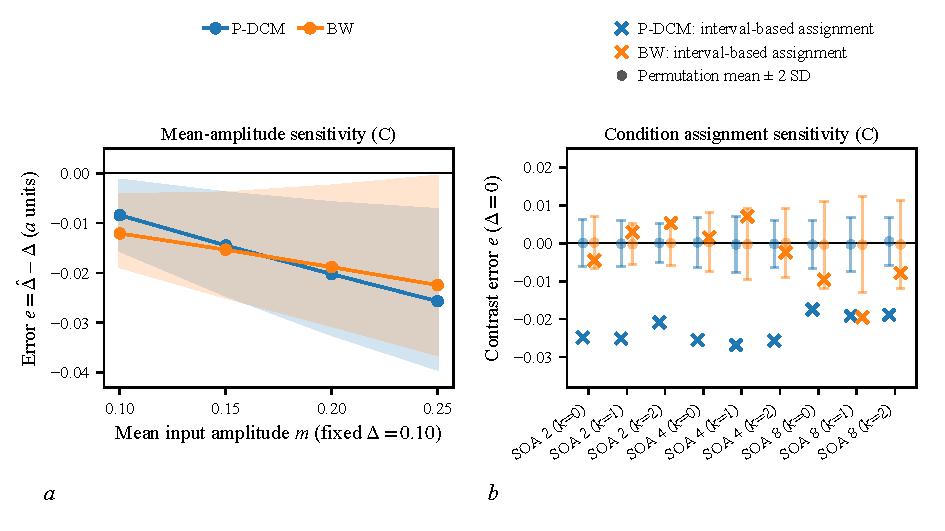
\includegraphics[width=15.5cm]{fig_6}
	\caption{Механизмы ошибки контраста для P-DCM и BW. \textit{a} --- медиана ошибки $e=\hat\Delta-\Delta$ по девяти последовательностям стимулов для $C$ и собственного $L_1$ при $a_B=a_A/2$; пунктир --- $\pm0{,}002$ модельной единицы. \textit{b} --- компоненты ошибки, предсказанные приближением второго порядка: фактическая нелинейная ошибка $e_{\mathrm{nl}}$, полная и статическая проекции. \textit{c} --- ошибка $C$ при росте средней амплитуды входного воздействия $m=(a_A+a_B)/2$ и фиксированном $\Delta=0{,}10$; полосы --- разброс min--max. \textit{d} --- ошибка $C$ при $a_A=a_B=0{,}20$ и $\Delta=0$: метки по истории событий и среднее $\pm2$ стандартных отклонения по 100 перестановкам; $k$ --- номер последовательности при данном среднем SOA. Обозначения на панелях: L1own --- собственное $L_1$, full Q --- полная квадратичная проекция, static Q --- статическая проекция.}
	\label{fig:f6}
\end{figure}

\subsection*{Полная поправка Вольтерра второго порядка}

Чтобы считать применение FV обоснованным, были заданы два условия: общее снижение RMSE контраста не менее $0{,}002$ и ухудшение в отдельном варианте условий не более $0{,}001$. Первое условие было выполнено: абсолютная RMSE уменьшилась на $\approx0{,}003$ (рис.~\ref{fig:f7}, \textit{a}). В основном классе ненулевых контрастов относительная RMSE снизилась с $28{,}7$ до $25{,}0\%$. Наибольшее снижение ошибки (примерно втрое) зафиксировано при среднем SOA 2~с. В единственной паре малого контраста $(0{,}2;\,0{,}18)$ применение FV увеличило ошибку: $53{,}1\%$ против $50{,}3\%$.

Второе условие не было выполнено: при изменении выходного усиления (рис.~\ref{fig:f7}, \textit{b}) в 40 тестовых последовательностях со средним SOA 8~с и усилениями $0{,}8$ и $1{,}25$ FV увеличила RMSE контраста во всех трех классах контраста. Этот результат получен прямым расчетом ожидания по известному распределению шума и не зависит от приближенных интервалов.

\begin{figure}[!t]
	\centering
	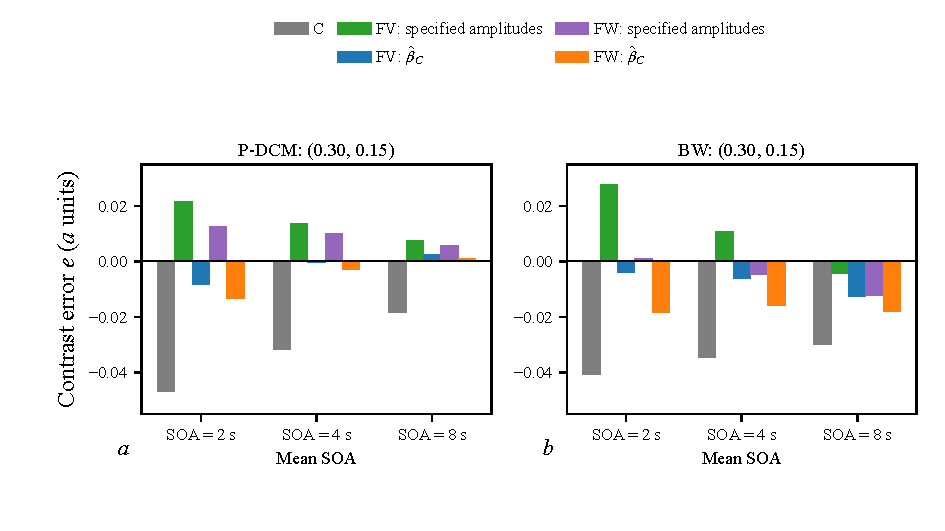
\includegraphics[width=16cm]{fig_7}
	\caption{Тестирование поправки FV: сводная RMSE и ухудшение по вариантам. \textit{a} --- RMSE контраста для $C$ и FV по четырем заранее заданным режимам и по всей совокупности. \textit{b} --- точечные оценки ухудшения точности $H_R=R_{\mathrm{FV}}-R_C$ и односторонние верхние границы для 36 заранее определенных вариантов (четыре режима, три класса контраста, три средних SOA); индексы 0--8, 9--17, 18--26 и 27--35 отвечают режимам Gain, Nominal, Parameter и Structure. Группа проходит условие, пока верхняя граница $H_R$ остается ниже красной линии --- допуска $0{,}001$. Верхние границы построены бутстрепом по последовательностям стимулов (1000 бутстреп-выборок) с нормальной аппроксимацией и поправкой Бонферрони при $\alpha=0{,}05$; $R$ --- RMSE контраста.}
	\label{fig:f7}
\end{figure}

\subsection*{Роль выходного усиления}

При выходном усилении $g$ заданный контраст $\Delta=a_A-a_B$ остается в исходной шкале. Линейные оценки меняются пропорционально $g$. Квадратичный вклад, вычисленный по оцененному входу, меняется пропорционально квадрату оценок, поэтому номинальная и фактическая нелинейность масштабируются по-разному. Диагностическим эталоном служит произведение усиления на заданный контраст, $g\Delta$. Этот эталон отделяет рассогласование выходной шкалы от нелинейного сжатия: ошибка относительно него равна $e_g=\hat\Delta-g\Delta=e-(g-1)\Delta$. Снижение ошибки относительно $g\Delta$ означает согласование с выходной шкалой, но при неизвестном $g$ модельную шкалу не восстанавливает: ошибка относительно $\Delta$ сохраняется.

Для режима $g=1{,}25$ и основного класса контрастов FV снизила RMSE относительно эталона $g\Delta$ примерно на три четверти: на $75{,}8\%$ без шума и на $76{,}0\%$ при SNR~8. При SNR~2 устойчивого улучшения нет.

\subsection*{Статическая поправка винеровского типа}

FW улучшала отдельные коэффициенты чаще, чем их разность, а подтвержденное улучшение контраста было достигнуто в меньшинстве вариантов (табл.~\ref{tab:fw}). Тестирование FW охватило 288 вариантов условий: сочетания генератора, варианта поправки (собственного или перенесенного), усиления, среднего SOA, амплитуд и уровня шума. В 144 вариантах без изменения усиления улучшение контраста подтверждено только в 28, причем во всех осталось частичным: после поправки ошибки не вошли в порог. В 102 вариантах порога не достигла ни одна из оценок, в остальных оценка с $C$ была достаточной до поправки либо исходы остались неразличимыми (табл.~\ref{tab:fw}). 

\begin{table}[h]
\caption{Распределение 144 вариантов без изменения усиления тестирования поправки FW по исходам для коэффициентов $\beta$ и контраста $A-B$. В скобках указано число вариантов с полным улучшением. Порог приемлемой ошибки $\delta_s=\max(0{,}002;\,0{,}05m_s)$ определен по масштабу $m_s$ каждого варианта}
\label{tab:fw}
\centering
\begin{tabular}{lcc}
\hline
Исход & Коэффициенты & Контраст $A-B$\\
\hline
Оценка с $C$ достаточна & 10 & 12\\
Улучшение подтверждено & 84 (8) & 28 (0)\\
Порог не достигнут ни одной оценкой & 43 & 102\\
Исходы не различимы & 7 & 2\\
\hline
\end{tabular}
\end{table}

В среднем по всем 288 вариантам FW почти не меняла ошибку коэффициентов: среднеквадратичная относительная ошибка оценок $\hat\beta_A$ и $\hat\beta_B$ составляет $25{,}3\%$ у $C$ и $25{,}2\%$ у FW. На всех уровнях шума различие между $C$ и FW не превышает $0{,}5$ процентного пункта, а при SNR~2 сама ошибка достигает трети амплитуды. В рассмотренных модельных условиях с высоким уровнем шума (SNR~2) FW не улучшала активационные оценки: улучшение контраста не подтверждено ни в одном из 96 вариантов. То же в вариантах малых амплитуд и в 72 вариантах с усилением $1{,}25$.

\subsection*{Границы второго порядка и оцененного входа}

Поправки FV и FW вычитают ошибку, предсказанную приближением второго порядка, поэтому их точность упирается в точность этого приближения. Приближение верно воспроизводит знак ошибки контраста всюду, где он различим, и ее величину примерно в двух третях случаев. Для каждого из двух генераторов проверено 45 сочетаний амплитуд, SOA и последовательностей стимулов, всего 90 сочетаний (рис.~\ref{fig:f8}). Знак считался различимым при абсолютной ошибке $0{,}002$ и выше одновременно в теоретическом и полном расчете. Таких сочетаний 67, и во всех знаки совпали. Критерий близости величины (расхождение не более $25\%$) выполнен в 62 из 90 случаев.

Предел приближения виден у P-DCM при $a_A=0{,}3$, $a_B=0{,}15$ и среднем SOA 2~с. Предсказание второго порядка составляет $-0{,}0615$ модельной единицы, фактическая ошибка полного генератора равна $-0{,}0468$. Остаток $+0{,}0147$ частично компенсирует квадратичный вклад, поэтому при сильной стимуляции предсказание завышает модуль нелинейной ошибки.

\begin{figure}[!ht]
	\centering
	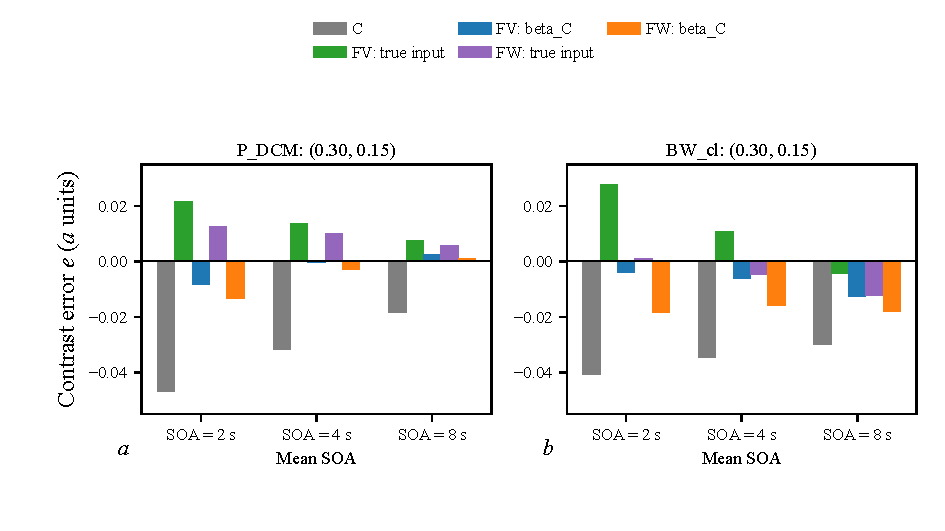
\includegraphics[width=16cm]{fig_8}
	\caption{Ошибки контраста $e=\hat\Delta-\Delta$ при $a_A=0{,}30$, $a_B=0{,}15$, основной последовательности ($k=0$) и средних SOA 2, 4 и 8~с для P-DCM (\textit{a}) и BW (\textit{b}). Столбцы --- каноническая оценка $C$, поправки FV и FW с входными амплитудами (теоретический контроль; при анализе реальных данных входные амплитуды неизвестны) и те же поправки с подстановкой оценок $\hat\beta_C$; обозначение beta\_C в легенде соответствует $\hat\beta_C$. Отдельная бесшумная диагностическая серия; со сводным тестированием FV и таблицей исходов FW она не объединяется.}
	\label{fig:f8}
\end{figure}
